\documentclass{article}

\usepackage[left=2cm,right=2cm, top=2cm, bottom = 2cm]{geometry}
\usepackage{amsfonts}

\usepackage{amsmath}
\usepackage{xcolor}

\usepackage{tikz}
\usepackage{subfigure}



\pagestyle{empty}

\setlength{\tabcolsep}{15pt}

\newcommand{\ihat}{\hat\i}
\newcommand{\jhat}{\hat\j}
\newcommand{\khat}{\hat{k}}





\begin{document}

\title{Linear Transformations}
\date{}

\maketitle
\thispagestyle{empty}

\Large

\textbf{\underline{Objective: To understand linear transformations of 2- and}}

\textbf{\underline{3-dimensional space and their representation as matrices.}}



\vspace{5mm}



\textbf{Warm-up:}\bigskip



Let's explore rotations of points about the origin.

\begin{enumerate}
\item Suppose the point $(1,0)$ is rotated anticlockwise by an angle $\theta$. What are its new coordinates?
\item Suppose the point $(0,1)$ is rotated anticlockwise by an angle $\theta$. What are its new coordinates?
\item Suppose the points $(1,0)$, $(0,1)$, and $(a,b)$ are rotated anticlockwise by $\frac{\pi}{2}$.
	\begin{enumerate}
	\item What are the coordinates of the rotations of $(1,0)$ and $(0,1)$?
	\item The rotated coordinates of $(a,b)$ are $(-b,a)$.
	We can relate the original coordinates to each other by the equation
	\[ (a,b) = a(1,0) + b(0,1).\]
	Write a similar equation linking the coordinates of the rotated points.
	\end{enumerate}
\item Suppose the points $(1,0)$, $(0,1)$, and $(a,b)$ are rotated anticlockwise by $\frac{3\pi}{4}$.
	\begin{enumerate}
	\item What are the coordinates of the rotations of $(1,0)$ and $(0,1)$?
	\item The rotated coordinates of $(a,b)$ are
	\[\left(\frac{-a}{\sqrt{2}}-\frac{b}{\sqrt{2}},\frac{b}{\sqrt{2}}-\frac{a}{\sqrt{2}}\right).\]
	We can relate the original coordinates to each other by the equation
	\[ (a,b) = a(1,0) + b(0,1).\]
	Write a similar equation linking the coordinates of the rotated points.
	\end{enumerate}
\end{enumerate}




\clearpage

\textbf{Theory---Rotations:}

\vspace{5mm}

Think of the point $(1,0)$ as instructions ``go one unit to the right.'' Call this instruction $\ihat$. Similarly, $(0,1)$ is the instruction ``go one unit upwards.'' Call this $\jhat$. Then a general point $(a,b)$ may be thought of as $a\ihat+b\jhat$---``go $a$ to the right and $b$ upwards.'' We call $\ihat$ and $\jhat$ the \textbf{standard unit vectors}.

\begin{center}
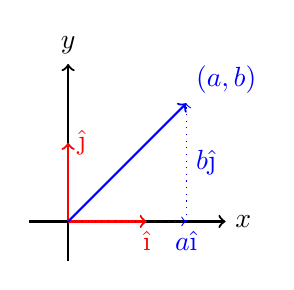
\begin{tikzpicture}
\draw[thick,->] (-0.5,0) -- (2,0);
\node[right] at (2,0) {$x$};
\draw[thick,->] (0,-0.5) -- (0,2);
\node[above] at (0,2) {$y$};

\draw[red,thick,->] (0,0) -- (1,0);
\node[below,red] at (1,0) {$\ihat$};
\draw[red,thick,->] (0,0) -- (0,1);
\node[right,red] at (0,1) {$\jhat$};

\draw[blue,thick,->] (0,0) -- (1.5,1.5);
\node[blue, above right] at (1.5,1.5) {$(a,b)$};
\draw[dotted,blue,->] (0,0) -- (1.5,0);
\node[blue, below] at (1.5,0) {$a\ihat$};
\draw[dotted,blue,->] (1.5,0) -- (1.5,1.5);
\node[blue,right] at (1.5,0.75) {$b\jhat$};
\end{tikzpicture}
\end{center}

Let $R$ denote rotation by an angle $\theta$. Then $R(\ihat)$ is the instruction ``move one unit in the direction $\theta$ above the positive $x$-axis'' and $R(\jhat)$ is the instruction ``move one unit in the direction $\theta$ anticlockwise of the positive $y$-axis.'' Rotate the whole setup above by $\theta$:

\begin{center}
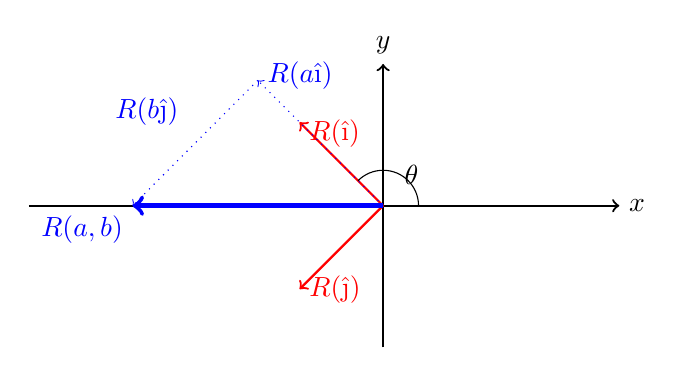
\begin{tikzpicture}[scale=1.5]
\draw[thick,->] (-3,0) -- (2,0);
\node[right] at (2,0) {$x$};
\draw[thick,->] (0,-1.2) -- (0,1.2);
\node[above] at (0,1.2) {$y$};

\draw[red,thick,->] (0,0) -- (-0.707,0.707);
\node[right,red] at (-0.707,0.607) {$R(\ihat)$};
\draw[red,thick,->] (0,0) -- (-0.707,-0.707);
\node[right,red] at (-0.707,-0.707) {$R(\jhat)$};
\draw (0.3,0) arc (0:135:0.3);
\node[above right] at (0.1,0.1) {$\theta$};

\draw[blue,ultra thick,->] (0,0) -- (-2.121,0);
\node[blue, below left] at (-2.121,0) {$R(a,b)$};
\draw[dotted,blue,->] (0,0) -- (-1.061,1.061);
\node[blue, right] at (-1.061,1.1) {$R(a\ihat)$};
\draw[dotted,blue,->] (-1.061,1.061) -- (-2.121,0);
\node[blue] at (-2,0.8) {$R(b\jhat)$};
\end{tikzpicture}
\end{center}

Rotating everything by $\theta$ doesn't affect the \textit{relative angles}. So if $R$ is any rotation, we have
\[R(a\ihat+b\jhat)=aR(\ihat)+bR(\jhat).\]

So to understand a rotation, it is enough to understand what it does to the \textbf{unit vectors} $\ihat$ and $\jhat$. We saw in the warm-up that, for rotation by angle $\theta$:
\[R(\ihat) = (\cos(\theta),\sin(\theta))=\cos(\theta)\ihat+\sin(\theta)\jhat\]
\[R(\jhat)=(-\sin(\theta),\cos(\theta))=-\sin(\theta)\ihat+\cos(\theta)\jhat.\]

Therefore we have:
\begin{align*}
R(a,b) &=aR(\ihat)+bR(\jhat)\\
&= a(\cos(\theta)\ihat+\sin(\theta)\jhat)+b(-\sin(\theta)\ihat+\cos(\theta)\jhat)\\
&= (a\cos(\theta)-b\sin(\theta))\ihat+(a\sin(\theta)+b\cos(\theta))\jhat\\
&=\left(a\cos(\theta)-b\sin(\theta),\; a\sin(\theta)+b\cos(\theta)\right)
\end{align*}

\clearpage


\textbf{Theory---Linear Transformations:}\bigskip


We saw on the last page that if $R$ is rotation by an angle $\theta$ anticlockwise about the origin, then for any point $(a,b)$:
\[R(a,b)=\left(a\cos(\theta)-b\sin(\theta),\; a\sin(\theta)+b\cos(\theta)\right).\]
Representing points by column vectors, we can write this as a matrix equation:
\[R\left(\begin{array}{c} a\\b\end{array}\right) = \left(\begin{array}{cc}\cos(\theta)&-\sin(\theta)\\\sin(\theta)&\cos(\theta)\end{array}\right)\left(\begin{array}{c}a\\b\end{array}\right).\]
Therefore the matrix
\[\left(\begin{array}{cc}\cos(\theta)&-\sin(\theta)\\\sin(\theta)&\cos(\theta)\end{array}\right)\]
gives a concise description of the rotation of any point about the origin.\medskip


The key to us showing this was that once you know what $R$ does to the standard unit vectors $\ihat$ and $\jhat$, then what it does to any other vector is determined by the equation
\[R(a,b)=aR(\ihat)+bR(\jhat).\]
This is because rotation about the origin is a \textbf{linear transformation}. A function $T$ from the plane to itself (or 3D space to itself, or in general any vector space to itself) is a \textbf{linear transformation} if it satisfies the two properties
\begin{align*}
	T(u+v)&=T(u)+T(v)\\
	T(\lambda v)&=\lambda T(v)
\end{align*}
for any vectors $u$ and $v$ and scalar $\lambda$.

\begin{enumerate}
	\item Let $A$ be a $2\times 2$ matrix and let $T_A:\mathbb{R}^2\to\mathbb{R}^2$ be the ``multiply by $A$'' function defined by $T_A(v)=Av$. Show that $T_A$ is a linear transformation.
	\item Let $T:\mathbb{R}^2\to\mathbb{R}^2$ be a linear transformation.
		\begin{enumerate}
			\item Show that for any point $(x,y)$, we have $T(x,y)=xT(\ihat)+yT(\jhat)$.
			\item Let $T(\ihat)=(a,c)$ and $T(\jhat)=(b,d)$. Show that (writing points as column vectors) $T$ is given by multiplication by the matrix
				\[\left(\begin{array}{cc} a & b\\c & d\end{array}\right).\]
		\end{enumerate}
\end{enumerate}

So multiplication by a matrix is a linear transformation, and any linear transformation can be written in this form! This is true in higher dimensions as well.


\clearpage

\textbf{Practice:}\bigskip

Rotation by angle $\theta$ anticlockwise about the origin:
\[\left(\begin{array}{cc}\cos(\theta)&-\sin(\theta)\\\sin(\theta)&\cos(\theta)\end{array}\right).\]
For any linear transformation $T$, if $T(1,0)=(a,c)$ and $T(0,1)=(b,d)$, then $T$ is represented by the matrix
\[\left(\begin{array}{cc} a & b\\c & d\end{array}\right).\]

\begin{enumerate}
	\item Calculate the inverse of the general rotation matrix above; compare with the rotation matrix by $-\theta$.
	\item Write down the matrices representing rotations about the origin by
		\begin{enumerate}
			\item $\frac{\pi}{4}$ anticlockwise
			\item $\frac{3\pi}{2}$ anticlockwise
			\item $\frac{\pi}{2}$ clockwise
			\item $\frac{2\pi}{3}$ clockwise
		\end{enumerate}
	\item Identify the rotation represented by the matrix
		\[\left(\begin{array}{cc} \frac{\sqrt{3}}{2}& \frac{1}{2}\\\frac{-1}{2} & \frac{\sqrt{3}}{2}\end{array}\right).\]
	\item Write down matrices representing the following linear transformations:
		\begin{enumerate}
			\item Reflection in the line $y=0$
			\item Reflection in the line $x=0$
			\item Reflection in the line $y=x$
			\item Reflection in the line $y=-x$
			\item Enlargement with scale factor 7 about the origin
			\item Contraction by $\frac{1}{3}$ about the origin
		\end{enumerate}
		and calculate their determinants.
	\item Describe the linear transformations represented by the following matrices:
		\[\left(\begin{array}{cc} 2 & 0\\ 0 & 1\end{array}\right),\quad \left(\begin{array}{cc} 1 & 0\\ 0 & \frac{1}{3}\end{array}\right),\quad \left(\begin{array}{cc} -5 & 0\\ 0 & 3\end{array}\right), \quad \left(\begin{array}{cc} \frac{3}{2} & 0\\ 0 & -7\end{array}\right).\]
\end{enumerate}

\clearpage


\textbf{Successive Transformations:}\bigskip

Suppose $S$ and $T$ are two linear transformations $\mathbb{R}^2\to\mathbb{R}^2$. Let $M_S$ and $M_T$ be the matrices representing them. Let $R:\mathbb{R}^2\to\mathbb{R}^2$ be the transformation defined by $R(v)=S(T(v))$; so $R$ is the result of doing first $T$ and then $S$. Show that the matrix representing $R$ is simply the matrix product $M_SM_T$.\bigskip


\begin{enumerate}
	\item Write down the matrices representing rotation by $45^\circ$ anticlockwise, and reflection in the line $y=-x$. Hence compute the matrices representing the compound transformations ``first rotate by $45^\circ$ anticlockwise, then reflect in the line $y=-x$'' and ``first reflect in $y=-x$, then rotate by $45^\circ$ anticlockwise.''
	\item Show that, for any angle $\theta$,
		\[\left(\begin{array}{cc} \cos(\theta)&-\sin(\theta)\\\sin(\theta)&\cos(\theta)\end{array}\right)\left(\begin{array}{cc}0&1\\1&0\end{array}\right)=\left(\begin{array}{cc}0&1\\1&0\end{array}\right)\left(\begin{array}{cc} \cos(\theta)&\sin(\theta)\\\sin(-\theta)&\cos(\theta)\end{array}\right).\]
		Hence conclude that reflecting the plane in the line $y=x$, then rotating by an angle $\theta$ anticlockwise is the same as first rotating by $\theta$ clockwise, then reflecting in $y=x$.
	\item Let $T\colon\mathbb{R}^2\to\mathbb{R}^2$ be a linear transformation and let $\lambda\in\mathbb{R}$ be a scalar. Show that first applying $T$ and then enlarging about the origin by a factor of $\lambda$ is the same as enlarging by $\lambda$ and then applying $T$. Note: this can be done using matrices, or the abstract definition of a linear transformation. Can you see both ways to do it?
	\item Let $\theta$ and $\phi$ be two angles. Let $R_\theta$, $R_\phi$, and $R_{\theta+\phi}$ be the rotations anticlockwise about the origin by the angles $\theta$, $\phi$, and $\theta+\phi$ respectively. Geometrically, we must have $R_{\theta+\phi}(v)=R_\theta(R_\phi(v))=R_\phi(R_\theta(v))$ for any vector $v$. Prove this using matrices.
	\item The matrix
		\[M=\left(\begin{array}{cc}\sqrt{3}&-1\\1&\sqrt{3}\end{array}\right)\]
		represents a rotation by $\theta$ followed by an enlargement by $\lambda$. Compute the determinant of $M$ and hence find the value of $\lambda$ (hint: the determinant is the \textit{area} scale factor, $\lambda$ is the \textit{length} scale factor). Hence find the value of $\theta$.
\end{enumerate}


\clearpage



\textbf{Linear Transformations of $\mathbb{R}^3$:}\bigskip

In $\mathbb{R}^2$, every point $(x,y)$ can be written as $x\ihat+y\jhat$, where $\ihat$ and $\jhat$ are the standard unit vectors. Similarly, in 3-dimensional space $\mathbb{R}^3$, we can define
\[\ihat=\left(\begin{array}{c}1\\0\\0\end{array}\right),\quad \jhat=\left(\begin{array}{c}0\\1\\0\end{array}\right),\quad \khat=\left(\begin{array}{c}0\\0\\1\end{array}\right),\]
and write any point $(x,y,z)$ as $x\ihat+y\jhat+z\khat$. Then, given a linear transformation $T\colon\mathbb{R}^3\to\mathbb{R}^3$, we have
\[T(x,y,z)=xT(\ihat)+yT(\jhat)+zT(\khat),\]
so $T$ is entirely determined by what it does to the three standard unit vectors. Given any $3\times 3$ matrix $A$, multiplication by $A$ (the function $T_A$ defined by $T_A(v)=Av$) is a linear transformation, and conversely any linear transformation $T$ can be written as $T_A$ where $A$ is the matrix
\[\left(\begin{array}{ccc}T(\ihat)&T(\jhat)&T(\khat)\end{array}\right),\]
whose columns are given by applying $T$ to the standard unit vectors. So just as in 2 dimensions, there is a correspondence between matrices and linear transformations.

\begin{enumerate}
	\item Describe the linear transformation represented by the matrix
		\[\left(\begin{array}{ccc}\cos(\theta) & -\sin(\theta)&0\\ \sin(\theta)&\cos(\theta)&0\\0&0&1\end{array}\right),\]
		where $\theta$ is any angle. Compute the determinant; does this make sense geometrically (in terms of volume scaling).
	\item Describe the linear transformation represented by the matrix
		\[\left(\begin{array}{ccc}\cos(\theta) &0& -\sin(\theta)\\0&1&0\\ \sin(\theta)&0&\cos(\theta)\end{array}\right),\]
		where $\theta$ is any angle.
	\item Write down the matrix representing a rotation about the $z$-axis by an angle $\theta$, anticlockwise in a right-handed coordinate system.
\end{enumerate}
\clearpage


\begin{enumerate}\setcounter{enumi}{3}
	\item Describe the linear transformations represented by the matrices
		\[\left(\begin{array}{ccc} -1&0&0\\0&1&0\\0&0&1\end{array}\right),\quad \left(\begin{array}{ccc} 1&0&0\\0&-1&0\\0&0&1\end{array}\right), \quad \left(\begin{array}{ccc} 1&0&0\\0&1&0\\0&0&-1\end{array}\right)\]
		and compute their determinants.
	\item Compute the matrix which represents a rotation of $60^\circ$ anticlockwise about the $z$-axis, followed by reflection in the plane $y=0$.
	\item Let $S$ be the linear transformation ``reflect in the plane $x=0$, then rotate by $\pi$ about the $y$-axis'' and let $T$ be the linear transformation ``reflect in the plane $z=0$.'' Compute the matrices $M_S$ and $M_T$ representing these transformations. What can you conclude about the transformations $S$ and $T$? What is the transformation ``do $S$, then do $T$?''
	\item Compute the matrix which represents reflection in the plane $z=0$, followed by rotation of $\frac{\pi}{2}$ about the $y$-axis, followed by rotation of $-\frac{5\pi}{3}$ about the $z$-axis, followed by reflection in the plane $x=0$.
	\item Let $R$ be the rotation about the $x$-axis by an angle $\frac{2\pi}{3}$ anticlockwise, and $S$ the reflection in the plane $y=0$. Let $M_R$ and $M_S$ be the matrices representing $R$ and $S$ respectively.
		\begin{enumerate}
			\item Compute $M_R^{-1}$ and $M_S^{-1}$ (hint: if you think about the geometry, you \textbf{don't} need to do any matrix calculations!).
			\item Compute the matrix representing the transformation ``do $R$, then do $S$.''
			\item Compute the inverse of the matrix from part (b).
			\item Compute the matrix products $M_R^{-1}M_S^{-1}$ and $M_S^{-1}M_R^{-1}$. Compare with your answer to part (c), and explain what you observe.
		\end{enumerate}
	\item Describe the linear transformation represented by the matrix
		\[\left(\begin{array}{ccc} 3&0&0\\ 0&\frac{1}{2}&0\\ 0&0&5\end{array}\right).\]
		Compute the determinant of this matrix and compare with what you would expect this transformation to do to volumes.
\end{enumerate}


\clearpage


\textbf{Further Practice:}\bigskip

These questions go beyond the A-level syllabus.

\begin{enumerate}
	\item Let $f\colon\mathbb{R}^2\to\mathbb{R}^3$ be the function defined by $f(x,y)=(x,y,x+y)$.
		\begin{enumerate}
			\item Viewing points as column vectors, write down $f(\ihat)$ and $f(\jhat)$ as column vectors, and create a $3\times 2$ matrix $A$ with these as columns.
			\item Compute
				\[A\left(\begin{array}{c}x\\y\end{array}\right)\]
				and compare with the definition of $f$.
			\item Show that $f$ is linear---\textit{i.e.}, that
				\[f(u+v)=f(u)+f(v)\quad\mbox{ and }\quad f(\lambda v)=\lambda f(v),\]
				for any scalar $\lambda$ and vectors $u$ and $v$.
		\end{enumerate}
	\item Let $g\colon\mathbb{R}^3\to\mathbb{R}^2$ be the function defined by $g(x,y,z)=(x,y)$.
		\begin{enumerate}
			\item Describe geometrically the effect of the function $g$.
			\item Show that $g$ is linear.
			\item Write down a $2\times 3$ matrix representing $g$.
			\item Let $f$ be the function from the previous question. Let $fg\colon\mathbb{R}^3\to\mathbb{R}^3$ denote the transformation ``first do $g$, then do $f$,'' so $fg(v)=f(g(v))$. Similarly, let $gf\colon\mathbb{R}^2\to\mathbb{R}^2$ be the transformation ``do $f$, then do $g$.'' Write down formulae expressing $fg$ and $gf$.
			\item Let $M_f$ be the $3\times 2$ matrix found in question 1, representing $f$, and let $M_g$ be the $2\times 3$ matrix representing $g$, found in part (c). Compute $M_fM_g$ and $M_gM_f$, and compare with your answers to part (d).
		\end{enumerate}
	\item Let $P$ be the set of all polynomials in the variable $x$ with real coefficients. Let $D\colon P\to P$ be the function ``differentiate with respect to $x$:'' so if $f$ is a polynomial, $D(f)$ is the derivative $f'(x)$.
		\begin{enumerate}
			\item Show that $D$ is linear---\textit{i.e.}, that for any two polynomials $f(x)$ and $g(x)$, and any scalar $\lambda$, we have
				\[D(f+g)=D(f)+D(g)\quad\mbox{ and }\quad D(\lambda f)=\lambda D(f).\]
			\item There are ``standard unit vectors'' in $P$: $1,x,x^2,x^3,\hdots,x^n,\hdots$, and every polynomial can be written in terms of finitely many of these ``standard unit vectors.'' Describe the effect of $D$ on a general one of these ``standard unit vectors.'' Hence write down the start of an ``infinite matrix'' representing the action of $D$.
		\end{enumerate}
	\item Recall that the \textbf{transpose} of a matrix is the matrix made by swapping its rows and columns (equivalently, reflecting in the leading diagonal). We say that an $n\times n$ matrix $M$ is \textbf{orthogonal} if $MM^T=I_n=M^TM$---\textit{i.e.}, if the transpose of $M$ is equal to the inverse of $M$.
		\begin{enumerate}
			\item Let $\theta$ be an angle; show that the matrix representing the rotation of $\mathbb{R}^2$ by an angle $\theta$ anticlockwise about the origin is an orthogonal matrix.
			\item Let $M$ be a general $2\times 2$ matrix; show that $|M|=|M^T|$.
			\item Let $M$ be a $2\times 2$ orthogonal matrix; show that $|M|=\pm 1$. You may assume for this question that $|AB|=|A|\times |B|$ for any $n\times n$ matrices $A$ and $B$; this is true, but hard to prove.
			\item Let $M$ and $N$ be orthogonal matrices. Show that $MN$ is also orthogonal (hint: $(MN)^T=N^TM^T$).
			\item Let $M$ be an orthogonal, $2\times 2$ matrix and let $N$ be the matrix representing reflection in the $y$-axis. Show that $MN$ is orthogonal and $|MN|=-|M|$.\medskip
			
			By part (c), every orthogonal matrix has determinant $\pm 1$. If $M$ is orthogonal and $|M|=+1$, we call $M$ \textbf{special orthogonal}. It can be shown that the special orthogonal matrices are precisely the rotation matrices! Moreover, part (e) shows that if $M$ is orthogonal but not special orthogonal (\textit{i.e.}, $|M|=-1$), then multiplying $M$ by reflection in the $y$-axis makes $M$ special orthogonal (any other reflection would also work for this). It follows that any orthogonal matrix is either special orthogonal (and so is a rotation matrix) or else represents reflection followed by a rotation. A reflection followed by a rotation is actually itself a reflection; so any orthogonal matrix is either a rotation or a reflection!
			
			This remains true in higher dimensions; the special orthogonal matrices are rotations, and the non-special orthogonal matrices are reflections, and can each be written as a single, fixed reflection, followed by a rotation. Once you see dot products, you will be able to prove that orthogonal matrices are precisely the linear transformations which preserve all lengths and angles. Putting that together with what we've looked at here: a linear transformation which preserves lengths and angles is either a rotation (if its determinant is $+1$) or a reflection (if its determinant is $-1$), and any reflection can be written as one fixed reflection followed by a rotation.
		\end{enumerate}
\end{enumerate}











\end{document}